% Front-matter for the M.Tech dissertation of Deepak Gupta (2024PCS0024).
% Declaration -> Approval Sheet -> Acknowledgement -> List of Publications.
% The Approval-of-the-DSC block is enabled only at viva-voce time by the DSC itself.

%=========================================================
% Declaration
\thispagestyle{plain}
\begin{center}
\textbf{\large DECLARATION}
\end{center}

This thesis is submitted as a requirement for the award of the Master of Technology degree in the Department of Computer Science and Engineering, Indian Institute of Technology Jammu. I declare that this written submission represents my ideas in my own words, and where others' ideas or words have been included, I have adequately cited and referenced the original sources. The research embodied in this thesis has not been submitted in part or in full to any other University or Institute for the award of any other degree or diploma before. I also declare that I have adhered to all principles of academic honesty and integrity and have not misrepresented, fabricated or falsified any idea/data/fact/source in my submission. Furthermore, I have not used any GenAI tools to generate the texts, except for grammatical checks and paraphrasing. I understand that any violation of the above will be a cause for disciplinary action by the Institute and can also evoke penal action from the sources that have not been properly cited, or from whom proper permission has not been obtained when required.

\vspace{1cm} \hfill
\begin{flushright}
	\IfFileExists{deepaksign.png}{%
		
\includegraphics[width=4.5cm,trim=0 220 0 60,clip,keepaspectratio]{deepaksign.png}\\[-0.6em]%
	}{%
		\vspace*{1.2cm}%
	}%
	\rule{7.0cm}{0.5pt} \\
	\hspace{2pt}Name: Deepak Gupta \\
	\hspace{2pt}Roll No.: 2024PCS0024
\end{flushright}

\newpage
\thispagestyle{empty}
\cleardoublepage

%=========================================================
% Approval Sheet
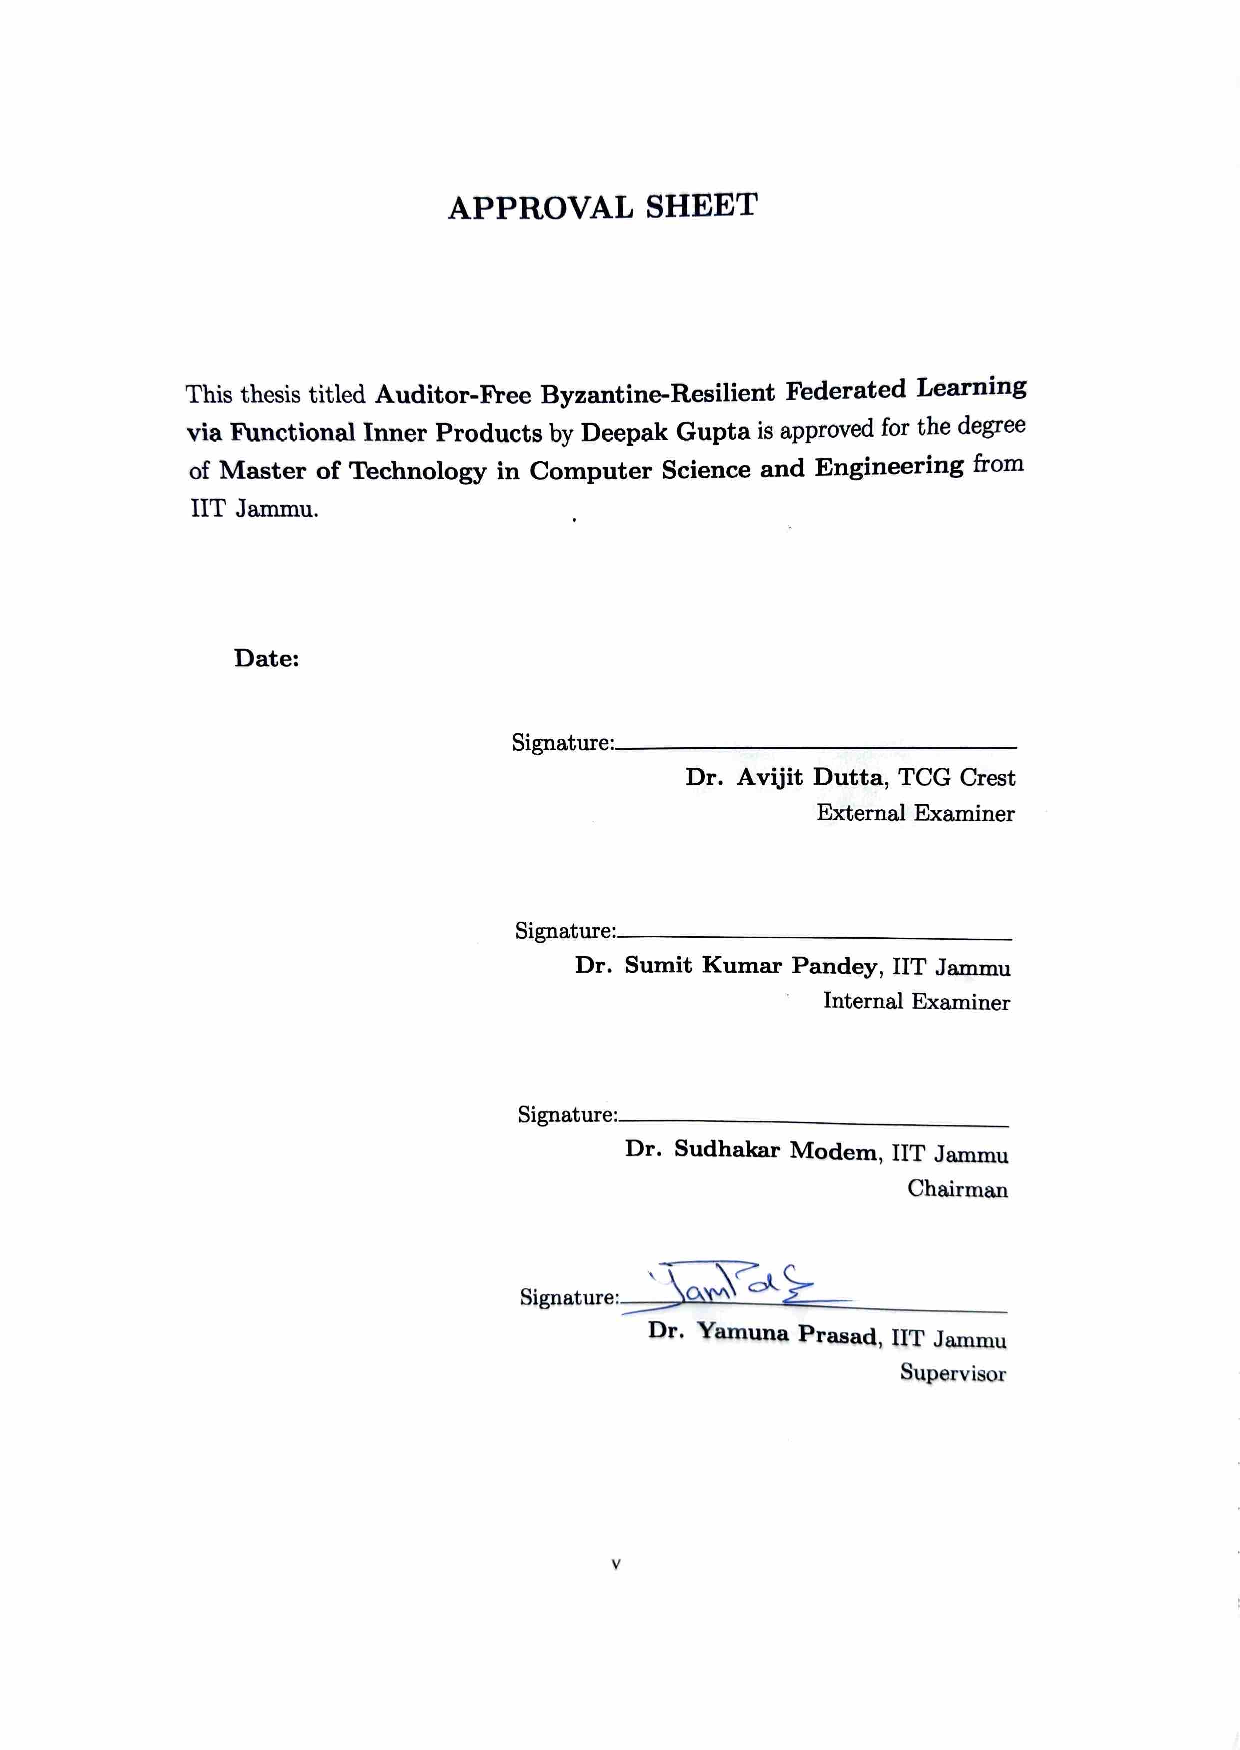
\includepdf[pages=1,pagecommand={\thispagestyle{empty}},width=\paperwidth,height=\paperheight,keepaspectratio]{approval_signed.pdf}

\newpage
\thispagestyle{empty}
\cleardoublepage

%=========================================================
% Dedication
\newpage
\thispagestyle{empty}
\vspace*{\fill}
\begin{center}
	\textit{\Large To my parents,}\\[0.4em]
	\textit{\Large who gave me the courage to dream big,}\\[0.4em]
	\textit{\Large and to my teachers,}\\[0.4em]
	\textit{\Large who showed me how to turn those dreams into reality.}
\end{center}
\vspace*{\fill}

\newpage
\thispagestyle{empty}
\cleardoublepage

%=========================================================
% Acknowledgement
\newpage
\thispagestyle{plain}
\begin{center}
\textbf{\Large Acknowledgement}
\end{center}

I want to record my thanks to the people who helped this dissertation reach its present form. The work passed through many small phases (problem reading, protocol drafts, experiment runs, and long revision cycles), and each of those phases was made easier by someone around me.

My deepest thanks go to my supervisor, Dr.~Yamuna~Prasad, Head of the Department of Computer Science and Engineering at IIT Jammu. Three areas feed into this thesis: privacy-preserving federated learning, applied cryptography, and adversarial machine learning. I genuinely do not think I could have tied them together without his guidance. Whatever coherence the final work has is in large part his doing. He let me follow my own ideas, but he rarely let a loose assumption pass; more than once he sent me back to justify a step or to repair a proof I had thought was finished. I learned a lot from working with him, as much from his patience as from the standard he sets for the work.

I am grateful, too, to the M.Tech and Ph.D. scholars at IIT Jammu who shared the lab and many long evenings with me. Whiteboard arguments, bugs we traced down together, and unhurried research conversations all helped shape parts of this work, and the months of writing and revision were a good deal less solitary for them.

The Department of Computer Science and Engineering at IIT Jammu provided the academic atmosphere, coursework, and the compute that this study needed; I thank the department, and all the faculty who taught me during the first year, for that support.

Finally, my parents and my family have stood behind me through every phase of this thesis; to them I owe far more than a line in an acknowledgement.

\vspace*{2mm}
\begin{flushright}
	\textbf{Deepak Gupta}
\end{flushright}

\newpage
\thispagestyle{empty}
\cleardoublepage

%=========================================================
% List of Publications (after Acknowledgement)
\newpage
\thispagestyle{plain}
\addcontentsline{toc}{chapter}{List of Publications}
\begin{center}
\textbf{\Large List of Publications}
\end{center}

\vspace{0.5cm}

\noindent \textbf{\large Conference Publications}
\begin{enumerate}
	\item Mahendra Kumar Gurve, Deepak Gupta, Nitin, and Yamuna Prasad, ``Eliminating the Auditor: Functional Inner Product Based Byzantine-Resilient Federated Learning,'' accepted as a poster at the \textit{ACM/IEEE International Conference on Embedded Artificial Intelligence and Sensing Systems (SenSys~2026)}, Saint-Malo, France, May 2026.
\end{enumerate}

\newpage
\thispagestyle{empty}
\cleardoublepage
